\chapter{PCA as a Data Analytic Tool}
	\label{c:3}
Principal component analysis (PCA) is a statistical procedure that uses an orthogonal transformation to convert a set of observations of possibly correlated variables into a set of values of linearly uncorrelated variables called principal components \cite{13}. The number of principal components is less than or equal to the smaller of the number of original variables or the number of observations. This transformation is defined in such a way that the first principal component has the largest possible variance and each succeeding component in turn has the highest variance possible under the constraint that it is orthogonal to the preceding components. As we can use PCA for dimensionality reduction, it can be used as a preprocessing step  in many machine learning algorithms that do not perform well with high-dimensional data. Therefore we can easily realize that PCA is an excellent tool for big data analysis. 

There are several ways to perform PCA. Eigen Value Decomposition (EVD) of covariance matrix and Singular Value Decomposition (SVD) are two basic and most common ways \cite{14}. These methods usually perform better on small datasets on a single machine. But in distributed settings and for big data, they introduce a new set of difficulties; they do not scale well to high dimensional data and are inefficient in terms of computation and communication cost \cite{elgamal}. To overcome these difficulties, two other methods, Stochastic SVD (SSVD) \cite{16} and Probabilistic PCA (PPCA) \cite{17} are used in practice. But unlike the other methods to calculate principal component (i.e. EVD of covariance matrix, SVD, SSVD), PPCA has two important advantages. It has the ability of handling missing data and calculating probabilistic model to generate synthesized data \cite{18}. These features are best suited for big data as missing values are prevalent in this case and a probabilistic model of the data will be more effective for analytical purposes.

Despite of being an excellent tool of data analysis, we lack in proper approach of PPCA in big data analysis. We saw a decent approach of making scalable PCA or \textit{sPCA} in a distributed environment  \cite{elgamal}.  It was designed for data analysis on large datasets on distributed commodity clusters. But unfortunately this approach is not capable of handling datasets with very large dimension, we can say data that is at the same time tall and wide. Moreover data sovereignty is not ensured. There was no method of performing PCA on big data located at different geographic location which involves independent computation at different clusters and accumulation of intermediate results. 

In this chapter, we will try to show in depth the various approaches of performing PCA with their advantages and disadvantages. Moreover we will show the very recent optimization on scalability of PPCA which is known as \textit{sPCA} with its special features and limitations.

\section{Assumptions Involved in PCA}
Mathematically, PCA is defined as on orthogonal linear transformation that transforms the data to a new coordinate system such that the greatest variance by some projection of the data comes to lie on the first coordinate (called the first principal component), the second gratest variance on the second coordinate and so on. Therefore, the assumptions involved in PCA are:

\begin{enumerate}
\item \textbf{Linearity}\\
Linearity vastly simplifies the problem by restricting the set of potential bases. With this
assumption PCA is now limited to re-expressing the data as a linear combination of its
basis vectors that is, we need to find the appropriate change of basis.
\item \textbf{Large variances have important structure}\\
This assumption also encompasses the belief that the data has a high Signal-to-Noise
Ratio ($SNR = \dfrac{\sigma_{signal}^2}{\sigma_{noise}^2}$). Hence, principal components with larger associated variances represent interesting structure, while those with lower variances represent noise.
Note that this is a strong, and sometimes, incorrect assumption.
\item \textbf{Orthogonal PCs}\\
This assumption provides an intuitive simplification that makes PCA soluble with linear algebra decomposition techniques.  
\end{enumerate}

\section{PCA and Change of Basis}
The goal of principal component analysis is to identify the most meaningful basis to re-express a data set. The hope is that this new basis will filter out the noise and reveal hidden structure. Determining this fact allows an experimenter to discern which dynamics are important, redundant or noise. 


With this rigor we may now state more precisely what PCA asks: \textit{Is there another basis, which is a linear combination of the original basis, that best re-expresses our data set?}


Let $\pmb{X}$ be the original data set, where each column is a single sample (or moment in time) of our data set.Here $\pmb{X}$ is a $D \times N$ matrix where $\pmb{N}$ in the number of samples and $\pmb{D}$ is the dimension of each sample. Let Y be another $D \times N$ matrix related by a linear transformation $\pmb{P}$. $\pmb{X}$ is the original recorded data set and $\pmb{Y}$ is a new representation of that data set.

\begin{equation}
\label{eq1}
\pmb{Y = PX}
\end{equation}
Also let us define the following quantities
\begin{itemize}
\item
 $\pmb{p_i}$ are the rows of $\pmb{P}$
 \item
 $\pmb{x_i}$ are the columns of $\pmb{X}$ 
 \item
 $\pmb{y_i}$ are the columns of $\pmb{Y}$
\end{itemize}


%\newpage
Equation \ref{eq1} represents a change of basis and thus can have many interpretations:
\begin{itemize}
\item $\pmb{P}$ is a matrix that transforms $\pmb{X}$ into $\pmb{Y}$
\item Geometrically, $\pmb{P}$ is a rotation and a stretch which again transforms $\pmb{X}$ into $\pmb{Y}$
\item The rows of $\pmb{P}$, $\{\pmb{p_1,p_2, \dots , p_D}\}$ are a set of new basis vectors for expressing the columns of $\pmb{X}$
\end{itemize}


The latter interpretation is not obvious but can be seen by writing out the explicit dot products of $\pmb{PX}$

\begin{align*}
\pmb{PX} &= 
\left[ \begin{array}{c}
\pmb{p_1} \\
\pmb{\vdots} \\
\pmb{p_D} 
\end{array}          \right]
\left[ \begin{array}{ccc}
\pmb{x_1} &\pmb{\hdots} &\pmb{x_N} \\
\end{array}          \right]
\\\pmb{Y} &= 
\left[ \begin{array}{ccc}
\pmb{p_1\cdot x_1} & \dots &\pmb{p_1\cdot x_N} \\
\vdots & \ddots &\vdots \\
\pmb{p_D\cdot x_1} & \dots &\pmb{p_N\cdot x_N} \\
\end{array}          \right]
\end{align*}

\newpage We can note the form of each column of  $\pmb{Y}$

$$\pmb{y_i} = 
\left[
\begin{array}{c}
\pmb{p_1 \cdot x_i}\\
\pmb{\vdots}\\
\pmb{p_D \cdot x_i}
\end{array}
\right]
$$

We recognize that each coefficient of $\pmb{y_i}$ is a dot-product of $\pmb{x_i}$ with the corresponding row in $\pmb{P}$. In other words, the $j^{th}$ coefficient of $\pmb{y_i}$ is a projection on to the $j^{th}$ row of $\pmb{P}$. This is in fact the very form of an equation where $\pmb{y_i}$ is a projection on to the basis of $\{\pmb{p_1, \hdots, p_D }\}$. Therefore, the rows of P are a new set of basis vectors for representing of columns of $\pmb{X}$.

By assuming linearity the problem reduces to finding the appropriate change of basis. The row vectors $\{\pmb{p_1, \hdots, p_D }\}$ in this transformation will become the principal components of $\pmb{X}$.. Several questions now arise:

\begin{itemize}
\item What is the best way to re-express $\pmb{X}$?
\item What is a good choice of basis $\pmb{P}$?
\end{itemize}

These questions must be answered by next asking ourselves what features we would like $\pmb{Y}$ to exhibit. Evidently, additional assumptions beyond linearity are required to arrive at a reasonable result. The selection of these assumptions is the subject of the next section.



\section{Eigenvalue Decomposition (EVD)}
Given a matrix $\textbf{Y}$ of size $N \times D$ ($N$ rows and $D$ columns), a PCA algorithm obtains $d$ principal components ($d \leq D$) that explain the most variance (and hence information) of the data in matrix $\textbf{Y}$ \cite{pca,kraska}. To be useful in practice, $d$ is chosen to be much smaller than $D$, that is $d \ll D$ . In case EVD technique, the target matrix $V$ is of dimension $N \times k$ where the columns of $V$ are the principal components of $\textbf{Y}$. 

\subsection{Covariance Matrix}
How do we quantify and generalize these notions to arbitrarily higher dimensions? Consider two sets of measurements with zero means:
$$A = \{a_1,a_2,...,a_N\} , B = \{b_1,b_2,...,b_N\}$$
where the subscript denotes the sample number. The variance
of $\pmb{A}$ and $\pmb{B}$ are individually defined as,
$$\sigma_A^2 = \dfrac{1}{N}\sum_i a_i^2$$
$$\sigma_B^2 = \dfrac{1}{N}\sum_i b_i^2$$
The covariance between  $\pmb{A}$ and $\pmb{B}$ is a straight-forward generalization.
$$covariance\ of\ \pmb{A}\ and\ \pmb{B} \equiv \sigma_{AB}^2 = \dfrac{1}{N}\sum
_i a_ib_i$$
The covariance measures the degree of the linear relationship between two variables. A large positive value indicates positively correlated data. Likewise, a large negative value denotes negatively correlated data. The absolute magnitude of the covariance measures the degree of redundancy. Some additional facts about the covariance:
\begin{itemize}
\item
$\sigma_{AB}$ is zero if and only if $\pmb{A}$ and $\pmb{B}$ are uncorrelated (e.g. Figure \ref{corel}, left panel)
\item
$\sigma^2_{AB} = \sigma^2_A\ if\ A = B$
\end{itemize}


\begin{figure}[!htbp]
\centering
\frame{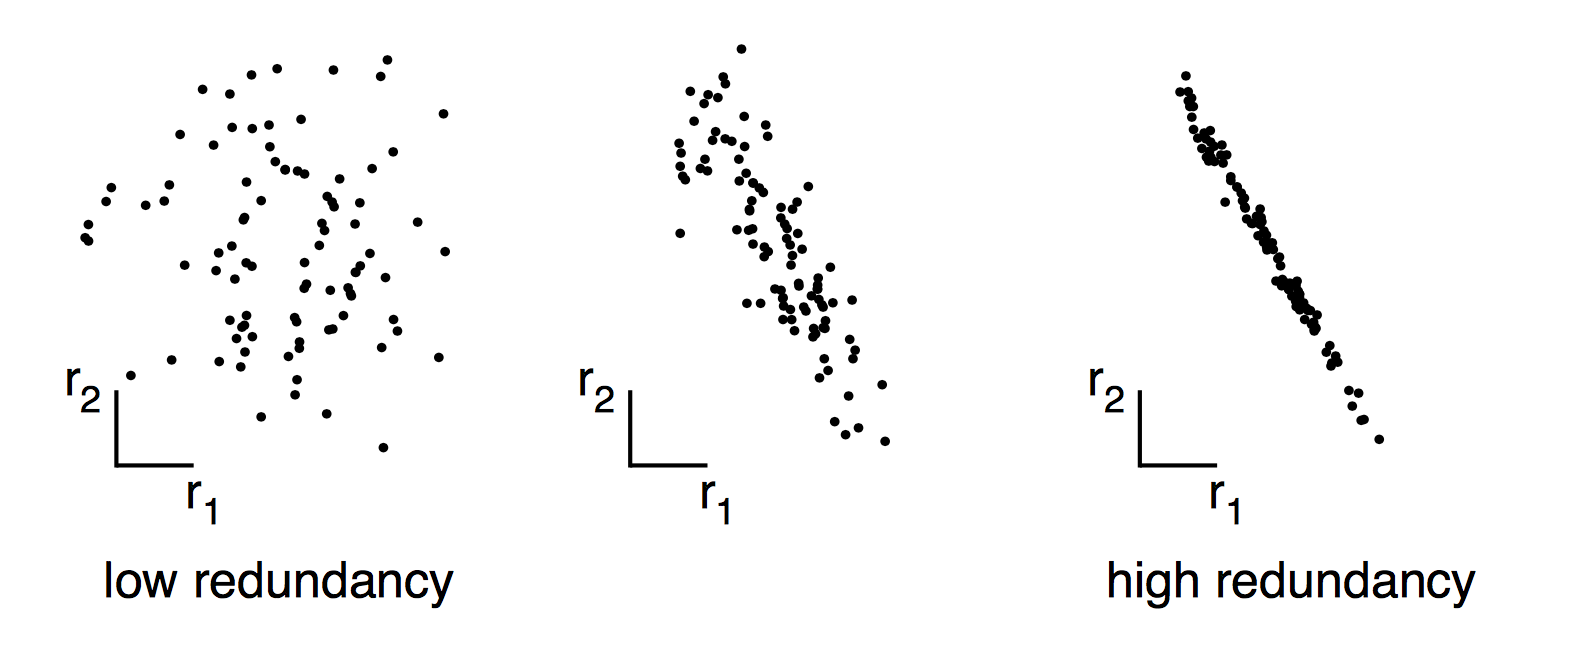
\includegraphics[scale=.5]{figures/corel}}
\caption{A spectrum of possible redundancies in data from the two separate measurements $r_1$ and $r_2$. The two measurements on the left are uncorrelated because one can not predict one from the other. Conversely, the two measurements on the right are highly correlated indicating highly redundant measurements.}
\label{corel}
\end{figure}

We can equivalently convert $\pmb{A}$ and $\pmb{B}$ into corresponding row
vectors.
\begin{align*}
\pmb{a} &= [a_1\ a_2\ \dots \ a_n]\\
\pmb{b} &= [b_1\ b_2\ \dots \ b_n]
\end{align*}
so that we may express the covariance as a dot product matrix computation
$$\sigma_{ab}^2 \equiv \dfrac{1}{N}\pmb{ab}^T$$
Finally, we can generalize from two vectors to an arbitrary number. Rename the row vectors a and $\pmb{b}$ as $\pmb{x_1}$ and $\pmb{x_2}$, respectively, and consider additional indexed row vectors $\pmb{x_1}$, $\dots$ , $\pmb{x_D}$. Define a new $D \times N$ matrix $\pmb{X}$.
$$ \pmb{X} = 
\left[ \begin{array}{c}
\pmb{x_1}\\\vdots\\\pmb{x_D}
\end{array}
\right]
$$
One interpretation of $\pmb{X}$ is the following. Each row of $\pmb{X}$ corresponds to all measurements of a particular type. Each column of $\pmb{X}$ corresponds to a set of measurements from one particular trial. We now arrive at a definition for the covariance matrix $\pmb{C_x}$

$$\pmb{C_x \equiv \dfrac{1}{N}XX}^T$$

Consider the matrix $\pmb{C_x = \dfrac{1}{N}XX}^T$ The $ij^{th}$ element of $\pmb{C_x}$ is the dot product between the vector of the ith measurement type with the vector of the $j^{th}$ measurement type. We can summarize several properties of $\pmb{C_x}$:
\begin{itemize}
\item $\pmb{C_x}$ is a square symmetric $D \times D$ matrix (Theorem 2 of Appendix \ref{ch:linear})
\item The diagonal terms of $\pmb{C_x}$ are the variance of particular measurement types
\item The off-diagonal terms of $\pmb{C_x}$ are the covariance between measurement types.
\end{itemize}
$\pmb{C_x}$ captures the covariance between all possible pairs of measurements. The covariance values reflect the noise and redundancy in our measurements.
\begin{itemize}
\item In the diagonal terms, by assumption, large values correspond to interesting structure
\item In the off-diagonal terms large magnitudes correspond to high redundancy
\end{itemize} 
Pretend we have the option of manipulating $\pmb{C_x}$. We will suggestively define our manipulated covariance matrix $\pmb{C_Y}$. What features do we want to optimize in $\pmb{C_Y}$?

\subsection{Diagonalize the Covariance Matrix}
We can summarize the last two sections by stating that our goals are

\begin{enumerate}
\item to minimize redundancy, measured by the magnitude of the covariance
\item maximize the signal, measured by the variance
\end{enumerate}  
What would the optimized covariance matrix $\pmb{C_Y}$ look like?
\begin{itemize}
\item All off-diagonal terms in $\pmb{C_Y}$ should be zero. Thus, $\pmb{C_Y}$ must be a diagonal matrix. Or, said another way, $\pmb{Y}$ is decorrelated
\item Each successive dimension in Y should be rank-ordered according to variance
\end{itemize} 
There are many methods for diagonalizing $\pmb{C_Y}$. It is curious to note that PCA arguably selects the easiest method: PCA assumes that all basis vectors $\{\pmb{p_1 , \dots , p_m} \}$ are orthonormal, i.e. $\pmb{P}$ is an orthonormal matrix.


\begin{figure}[!htbp]
\centering
\frame{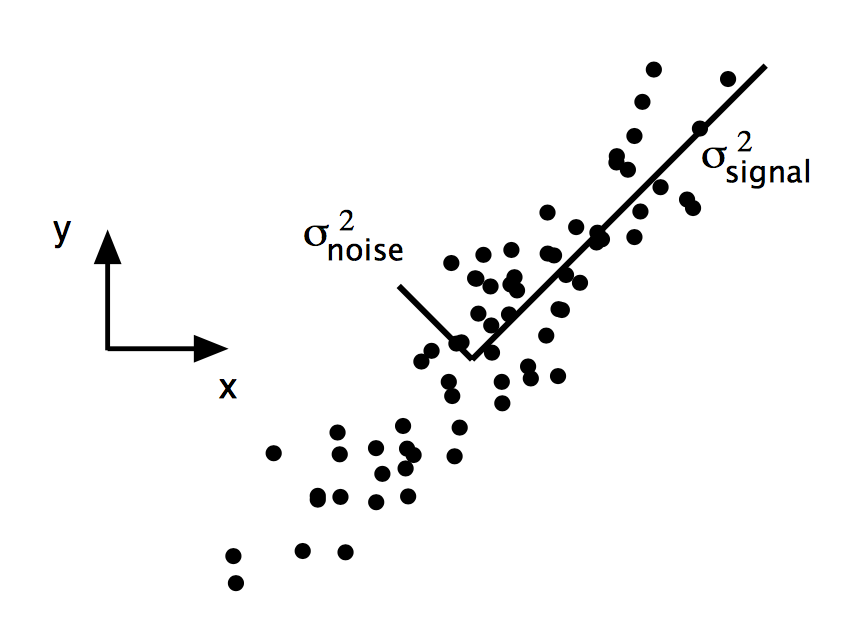
\includegraphics[scale=.6]{figures/fig2}}
\caption{A typical 2D example. The signal and noise variances $\sigma^2_{signal}$ and $\sigma^2_{noise}$ are graphically represented by the two lines subtending the cloud of data. The largest direction of variance lie along the best-fit line}
\label{fig2}
\end{figure}

 In a simple $2D$ example like in Figure \ref{fig2}, $\pmb{P}$ acts as a generalized rotation to align a basis with the axis of maximal variance. In multiple dimensions this could be performed by a simple algorithm:
 \begin{enumerate}
\item Select a normalized direction in m-dimensional space along which the variance in $\pmb{X}$ is maximized. Save this vector as $\pmb{p_1}$ .
\item Find another direction along which variance is maximized, however, because of the orthonormality condition, restrict the search to all directions orthogonal to all previous selected directions. Save this vector as $\pmb{p_2}$
\item Repeat this procedure until $D$ vectors are selected.
 \end{enumerate}
The resulting ordered set of $\pmb{p}$'s are the principal components.




\subsection{Solving PCA in EVD Approach}
We derive our first algebraic solution to PCA based on an important property of eigenvector decomposition. Once again, the data set is $\pmb{P}$, an $D \times N$ matrix, where $D$ is the number of measurement types and $N$ is the number of samples. The goal is summarized as follows

\begin{center}
\begin{tabular}{p{12cm}}
Find some orthonormal matrix $\pmb{P}$ in $\pmb{Y = PX}$ such that $\pmb{C_Y \equiv \dfrac{1}{N}XX}^T$ is a diagonal matrix. The rows of  $\pmb{P}$  are the principal components of  $\pmb{X}$ 
\end{tabular}
\end{center}
We begin by rewriting $\pmb{C_Y}$ in terms of the unknown variable

\begin{align*}
\pmb{C_Y} &= \dfrac{1}{N}\pmb{YY}^T\\
&= \dfrac{1}{N}\pmb{(PX)(PX)}^T\\
&= \dfrac{1}{N}\pmb{PXX}^T\pmb{P}^T\\
&= \pmb{P}(\dfrac{1}{N}\pmb{XX}^T)\pmb{P}^T\\
\pmb{C_Y} &= \pmb{PC_XP}^T 
\end{align*}

Note that we have identified the covariance matrix of $\pmb{X}$  in the last line.

Our plan is to recognize that any symmetric matrix A is diagonalized by an orthogonal matrix of its eigenvectors (by Theorems 3 and 4 from Appendix \ref{ch:linear}). For a symmetric matrix $\pmb{A}$  Theorem 4 provides $\pmb{A = EDE}^T$, where $\pmb{D}$  is a diagonal matrix and $\pmb{E}$  is a matrix of eigenvectors of $\pmb{A}$  arranged as columns.

Now we comes the trick. We select the matrix $\pmb{P}$  to be a matrix where each row $\pmb{p_i}$  is an eigenvector of $\dfrac{1}{N}\pmb{XX}^T$ . By this selection, $\pmb{P \equiv E}^T$ . With this relation and Theorem 1 of Appendix \ref{ch:linear} ($\pmb{P}^{-1} = \pmb{P}^T$) we can finish evaluating $\pmb{C_Y}$.

\begin{align*}
\pmb{C_Y} &= \pmb{PC_XP}^T\\
&= \pmb{P(E}^T\pmb{DE)P}^T\\
&= \pmb{P(P}^T\pmb{DP)P}^T\\
&= \pmb{(PP}^T)\pmb{D(PP)}^T\\
&= \pmb{(PP}^{-1})\pmb{D(PP)}^{-1}\\
\pmb{C_Y} &= \pmb{D}
\end{align*}

It is evident that the choice of $\pmb{P}$ diagonalizes $\pmb{C_Y}$. This was the goal for PCA. We can summarize the results of PCA in the matrices $\pmb{P}$ and $\pmb{C_Y}$.

\begin{itemize}
\item The principal components of $\pmb{C_Y}$ are the eigenvectors of $\pmb{C_X}$ = $\dfrac{1}{N}\pmb{XX}^T$
\item The $i^{th}$ diagonal value of $\pmb{C_Y}$ is the variance of $\pmb{X}$ along $\pmb{p_i}$
\end{itemize}

\section{Practical Approach of EVD}
In practice computing PCA of a data set $\pmb{X}$ is done in two steps:
\begin{enumerate}
\item subtracting off the mean of each measurement type 
\item computing the eigenvectors of $\pmb{C_X}$
\end{enumerate}
\section{Singular Value Decomposition (SVD)}
Let $\textbf{X}$ be an arbitrary $N \times D$ matrix and $\pmb{X}^T\pmb{X}$ be a rank $r$, square, symmetric $D \times D$ matrix. 

\subsection{Performing SVD}
To do Singular Value Decomposition of matrix \textbf{X} let us assume that:
\begin{itemize}
\item $\{\hat{v} _1,\hat{v} _2, \dots ,\hat{v} _r\}$ is the set of orthonormal $D \times 1$ eigenvectors with associated eigenvalues $\{\lambda _1, \lambda _2, \dots, \lambda _r\}$ for the symmetric matrix $\pmb{X^TX}$
$$(  \pmb{X^TX} ) \hat{v} _i = \lambda _i\hat{v} _i$$

\item
$\sigma_i \equiv \sqrt{\lambda_i}$ are positive real and termed the singular values.

\item 
$\{\hat{u} _1,\hat{u} _2, \dots ,\hat{u} _r\}$ is the set of $N \times 1$ vectors defined by $\pmb{\hat{u}_i \equiv \dfrac{1}{\sigma_i}X\hat{v}_i}$

\begin{equation}
\label{eq3}
\pmb{\sigma_i\hat{u}_i \equiv X\hat{v}_i}
\end{equation}

\end{itemize}

This result says a quite a bit. $\pmb{X}$ multiplied by an eigenvector of $\pmb{X^TX}$ is equal to a scalar times another vector. We can summarize this result for all vectors in one matrix multiplication by following the prescribed construction in Figure \ref{SVD}. We start by constructing a new diagonal matrix $\sum$.

$$\pmb{
\sum \equiv
\left[
    \begin{array}{cccccc}
    \sigma_1                                    \\
    & \ddots & & &\text{\huge0}\\
	& & \sigma_{\tilde{r}} \\
	& & &0 \\
	& \text{\huge0} &  & &\ddots             \\
      &               &   &   &  & 0
    \end{array}
    \right]
    }
$$

where $\sigma_{\tilde{1}} \geq \sigma_{\tilde{2}} \geq  \dots \geq \sigma_{\tilde{r}}$ are the rank-ordered set of singular values. Likewise we construct accompanying orthogonal matrices,
$$\pmb{V} = 
	\left[
	\begin{array}{cccc}
	\pmb{\hat{v}_{\tilde{1}}} &\pmb{\hat{v}_{\tilde{2}}} & \dots &\pmb{\hat{v}_{\tilde{D}}}
	\end{array}
	\right]
$$   
$$ \pmb{U} = 
	\left[
	\begin{array}{cccc}
	\pmb{\hat{u}_{\tilde{1}}} &\pmb{\hat{u}_{\tilde{2}}} & \dots &\pmb{\hat{u}_{\tilde{N}}}
	\end{array}
	\right]
$$   

where we have appended an additional ($D - r$) and ($N - $r) orthonormal vectors to ``fill up'' the matrices for \textbf{V} and \textbf{U} respectively (i.e. to deal with degeneracy issues).
 Figure \ref{SVD} provides a graphical representation of how all of the pieces fit together to form the matrix version of \textit{SVD}.
$$\pmb{XV = U\sum}$$
where each column of $\pmb{V}$ and $\pmb{U}$ perform the scalar version of the decomposition (Equation \ref{eq3}). Because $\pmb{V}$ is orthogonal, we can multiply both sides by $\pmb{V^1}$ = $\pmb{V}^T$ to arrive at the final form of the decomposition.
\begin{equation}
\label{eq4}
\pmb{X = U \sum V}^T 
\end{equation}
Although derived without motivation, this decomposition is quite powerful. Equation \ref{eq4} states that any arbitrary matrix \textbf{X} can be converted to an orthogonal matrix, a diagonal matrix and another orthogonal matrix (or a rotation, a stretch and a second rotation)


\begin{figure}
\centering
\frame{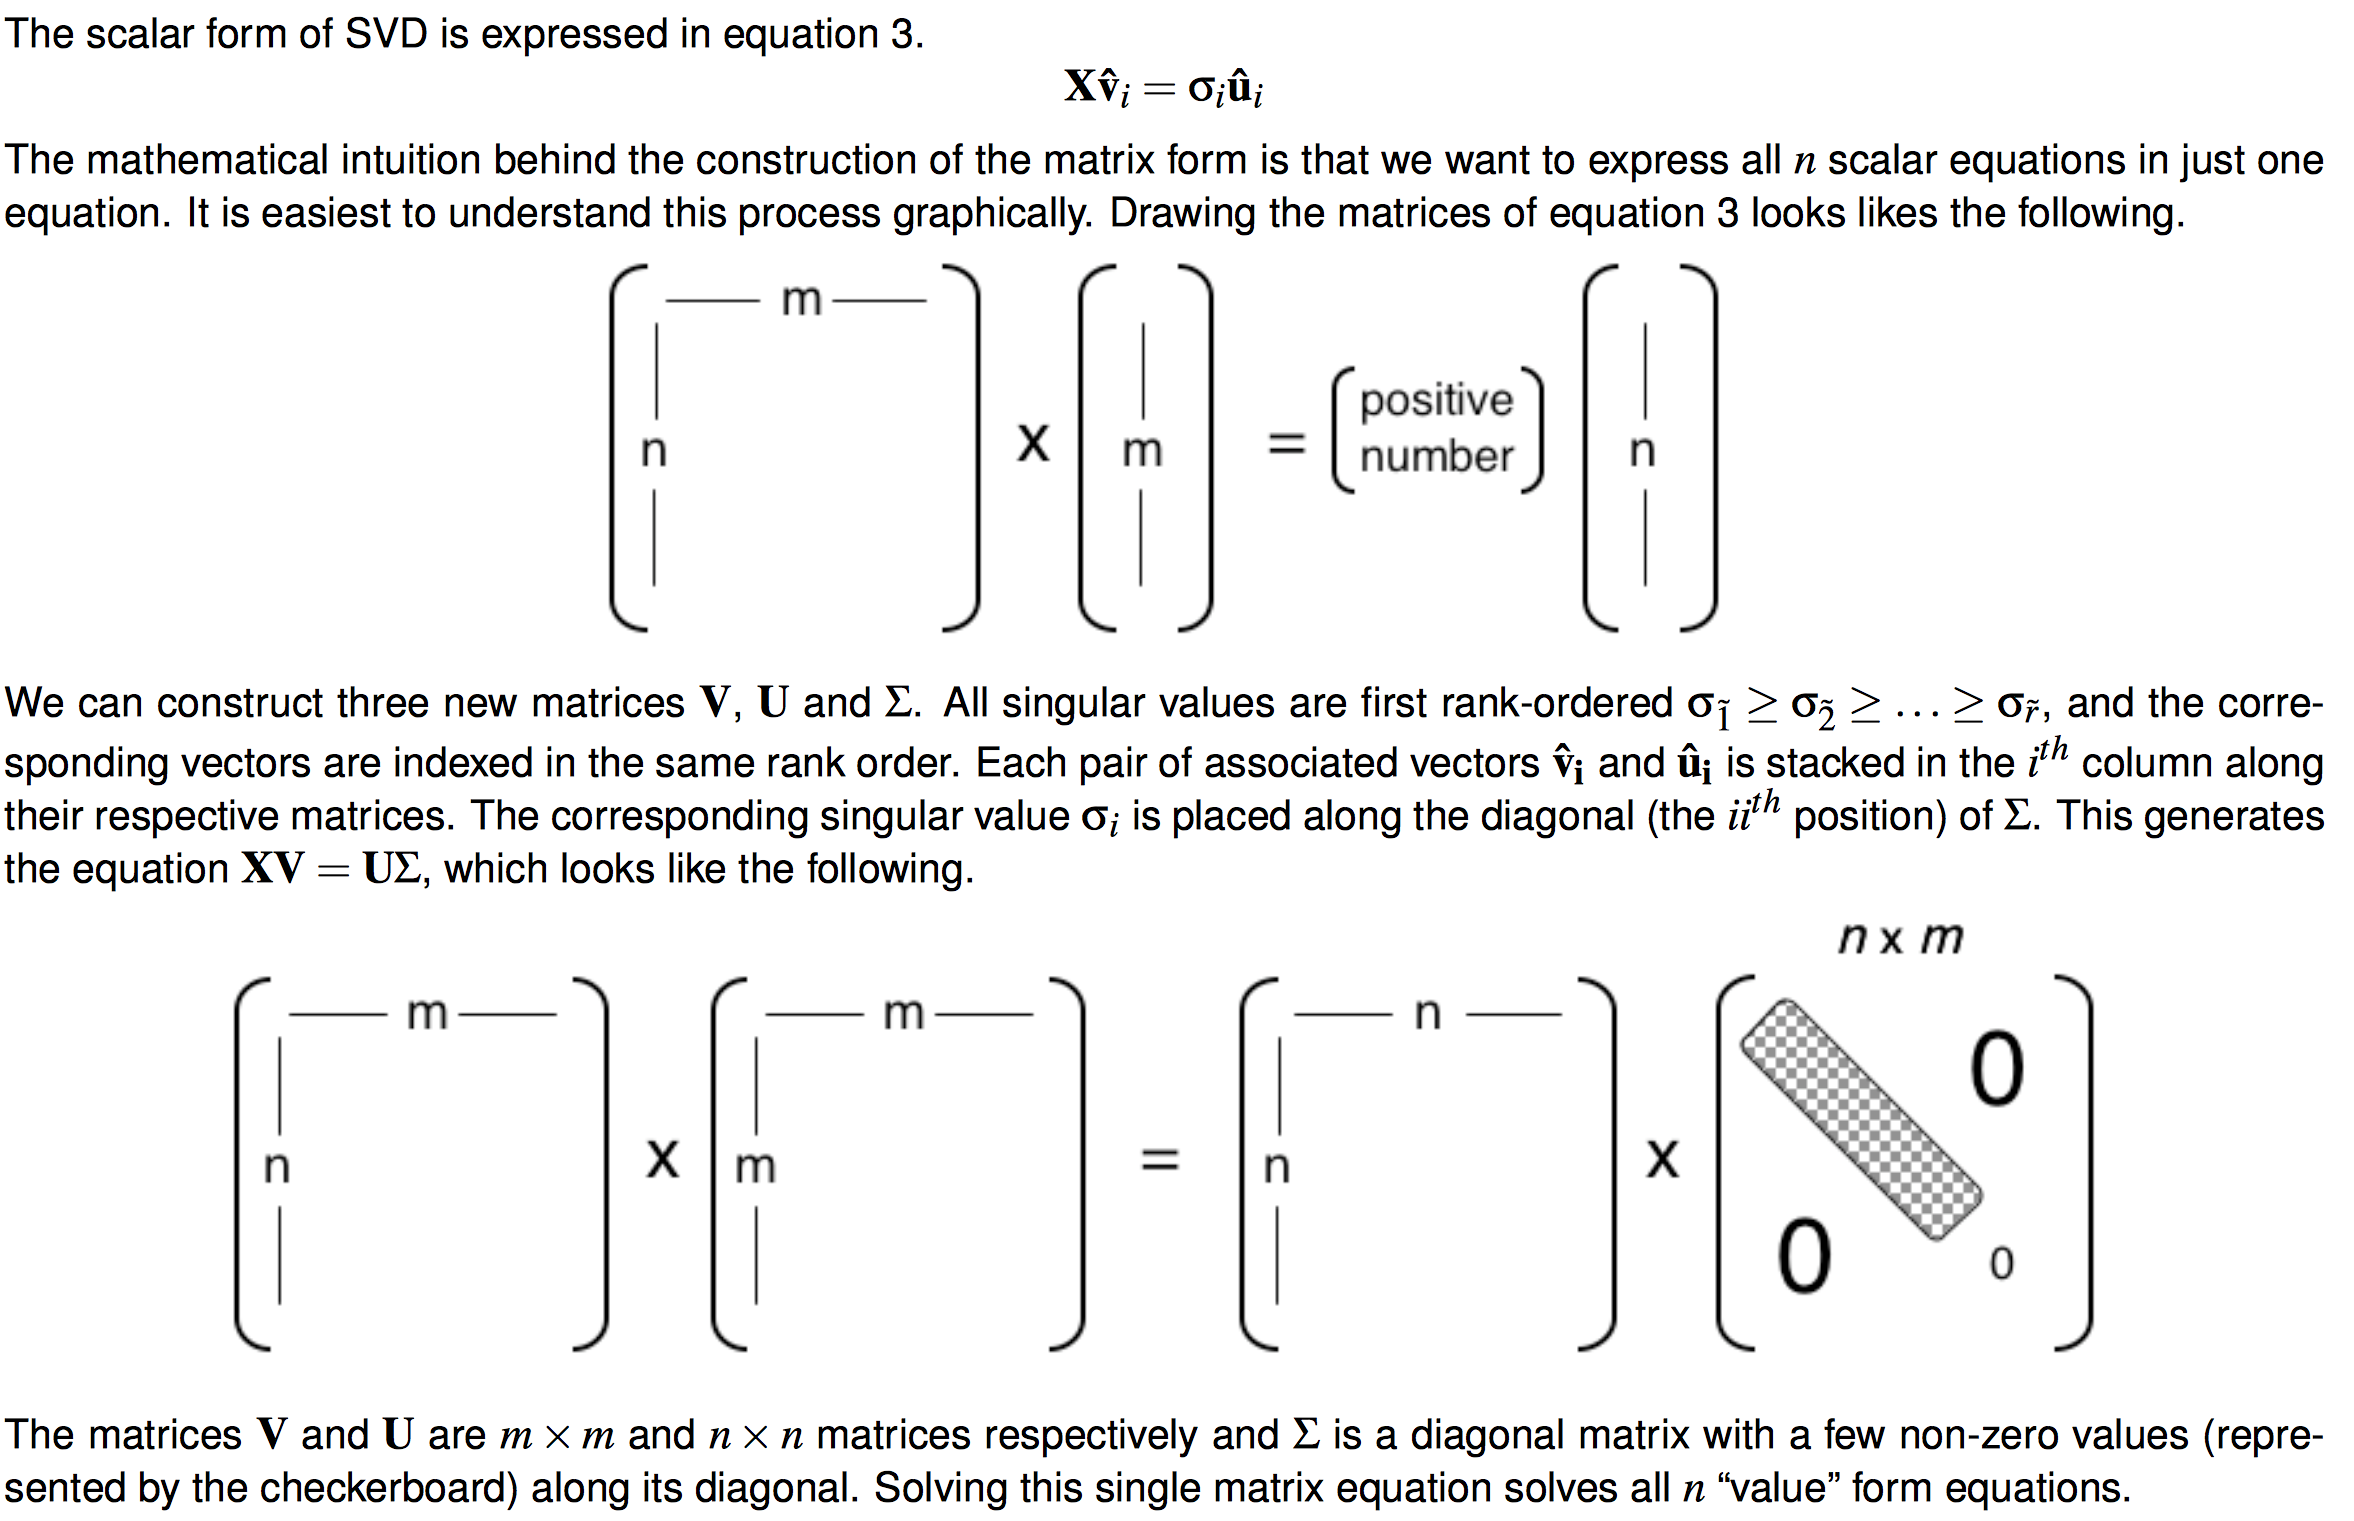
\includegraphics[scale=.38]{figures/SVD}}
\caption{Construction of the matrix form of SVD \ref{eq4} from the scalar form \ref{eq3}}
\label{SVD}
\end{figure}

\subsection{Linking SVD with EVD}

How does this link in to the previous \textit{EVD} analysis of PCA? Let us consider the $N \times D$ matrix, \textbf{X}, for which we have a singular value decomposition, $\pmb{X = U \sum V}^T$. There is a theorem from linear algebra which says that the non-zero singular values of \textbf{X} are the square roots of the nonzero eigenvalues of $\pmb{AA}^T$ or $\pmb{A}^T\pmb{A}$. 

\newpage The former assertion for the case $\pmb{A}^T\pmb{A}$ is proven in the following way:
\begin{align*}
\pmb{A}^T\pmb{A}  &= (\pmb{U\sum V}^T)^T(\pmb{U\sum V}^T)\\
										   &= (\pmb{V\sum}^T\pmb{U}^T)(\pmb{U\sum V}^T)\\
										   &= \pmb{V}(\sum^T\sum)\pmb{V}^T
\end{align*}

We observe that $\pmb{A}^T\pmb{A}$ is similar to $\sum^T\sum$ and thus it has the same eigenvalues. Since $\sum^T\sum$ is a square ($D \times D$), diagonal matrix, the eigenvalues are in fact the diagonal entries, which are the squares of the singular values. Note that the non-zero eigenvalues of each of the covariance matrices, $\pmb{AA}^T$ and $\pmb{A}^T\pmb{A}$ are actually identical.


It should also be noted that we have effectively performed an eigenvalue decomposition for the matrix, $\pmb{A}^T\pmb{A}$. Indeed, since AT A is symmetric, this is an orthogonal diagonalisation and thus the eigenvectors of $\pmb{A}^T\pmb{A}$ are the columns of $\pmb{V}$. This will be important in making the practical connection between the SVD and and the PCA of matrix X, which is what we will do next.


Returning to the original $N \times D$ data matrix, $\pmb{X}$, let us define a new $D \times N$ matrix, $\pmb{Z}$:

$$\pmb{Z} = \dfrac{1}{\sqrt{N-1}}\pmb{X}^T$$

Recall that since the m rows of $\pmb{X}$ contained the $N$ data samples, we subtracted the row average from each entry to ensure zero mean across the rows. Thus, the new matrix, $\pmb{Z}$ has columns with zero mean. Consider forming the $D \times D$ matrix, $\pmb{Z}^T\pmb{Z}$:
\begin{align*}
\pmb{Z}^T\pmb{Z} &= (\dfrac{1}{\sqrt{N-1}}\pmb{X}^T)^T(\dfrac{1}{\sqrt{N-1}}\pmb{X}^T)\\
&= \dfrac{1}{N-1}\pmb{XX}^T\\
i.e. \  \pmb{Z}^T\pmb{Z} &= \pmb{C_x}
\end{align*}
We find that defining $\pmb{Z}$ in this way ensures that $\pmb{Z}^T\pmb{Z}$ is equal to the covariance matrix of $\pmb{Z}$, $\pmb{C_x}$. From the discussion in the previous section, the principal components of $\pmb{X}$ (which is what we are trying to identify) are the eigenvectors of $\pmb{C_x}$. Therefore, if we perform a singular value decomposition of the matrix $\pmb{Z}^T\pmb{Z}$, the principal components will be the columns of the orthogonal matrix, $\pmb{V}$.

The last step is to relate the \textit{SVD} of $\pmb{Z}^T\pmb{Z}$ back to the change of basis:

$$\pmb{Y} = \pmb{PX}$$

We wish to project the original data onto the directions described by the principal components. Since we have the relation $\pmb{V} = \pmb{P}^T$ , this is simply: 

$$\pmb{Y} = \pmb{V}^T\pmb{X}$$

If we wish to recover the original data, we simply compute (using orthogonality of $\pmb{V}$): 

$$\pmb{X} = \pmb{VY}$$

\subsection{SVD for Dense Matrices}


Golub and Kahan \cite{golub} introduced a two-step approach for computing SVD: convert the input matrix to a bidiagonal one and then perform SVD on the bidiagonal matrix. Demmel and Kahan \cite{demmel} improved this approach by adding another step before bidiagonalization, which is QR decomposition. \cite{elgamal} refered to this method as SVD-Bidiag, which has the following three steps for a given matrix $\pmb{Y}$:
\begin{enumerate}
\item
compute the QR decomposition of $\pmb{Y}$, which results in an orthogonal matrix \textbf{Q} and an upper triangular matrix $\pmb{R}$ 

\item
transform \textbf{R} to a bidiagonal matrix $\pmb{B}$
\item 
compute SVD on $\pmb{B}$
\end{enumerate}
The SVD-Bidiag algorithm is implemented in \textit{RScaLAPACK}. Their analysis showed that the computational complexity of the SVD-Bidiag algorithm is dominated by the QR decomposition and bi-diagonalization steps, and is given by $\mathcal{O}(ND^2 + D^3)$. Therefore, the SVD-Bidiag algorithm is only suitable when D is small. More details can be found in \cite{elgamal}.

\subsection{SVD for Sparse Matrices}
SVD can be computed efficiently for sparse matrices using Lanczos' algorithm \cite{roman}, which has a computational complexity of $\mathcal{O}(Nz^2)$, where $z$ is the number of non-zero dimensions (out of \textbf{D} dimensions). More details can be found in \cite{elgamal}.


\section{Stochastic SVD (SSVD)}
Randomized sampling techniques have recently gained popularity in solving large-scale linear algebra problems. The work in \cite{halko} describes a randomized method to compute approximate decomposition of matrices, which is referred to as stochastic SVD (SSVD). SSVD has two steps: 
\begin{enumerate}
\item It uses randomized techniques to compute a low-dimensional approximation of the input matrix
\item It performs SVD on the approximation matrix
\end{enumerate}
The accuracy of the results depends on the performance of the randomized techniques and the size of the approximation matrix. Accuracy can be improved through running the randomization step multiple times. Therefore, SSVD has the flexibility of trading off the accuracy of the results with the required computational resources.

\section{Computational Complexity}
Computational complexity of SSVD is dominated by the first step, which is $\mathcal{O}(DNd)$. This is a much better complexity than the previous techniques, because $d$ is typically much smaller than $D$ and is usually a constant. However, SSVD requires exchanging multiple intermediate matrices, which may cause a problem for scalability. The amount of intermediate data can be up to $\mathcal{O}(max(Nd,d2))$ \cite{elgamal}.
\section{Probabilistic PCA (PPCA)}
We will be trying to present \textit{PPCA} in some kind of detail. For this we will follow the research work of Tipping and Bishop \cite{bishop}
\subsection{What is PPCA}
We can obtain a probabilistic formulation of PCA by introducing a Gaussian latent i.e. unobserved variable model. This kind of model is highly related to statistical factor analysis. First let us define some quantity:
\begin{itemize}
\item $\pmb{y}$ is a $D$ dimensional observed data vector
\item $\pmb{x}$ is a $d$ dimensional latent variable
\item $\pmb{W}$ is a $D \times d$ transformation matrix
\item the columns of $\pmb{W}$ are the principal components
\item $\pmb{\mu}$ is the dimension wise mean vector of $\pmb{y}$. This parameter allows the data to have non zero mean
\item $\pmb{\epsilon}$ is a $D$-dimensional zero-mean  noise variable
\item Here $\pmb{x}$, $\pmb{\epsilon}$, $\pmb{y}$ are normal distributed i.e. Gaussian distributed
\begin{align*}
\pmb{x} &\sim \mathcal{N}(\pmb{0},\pmb{I})\\
\pmb{\epsilon} &\sim \mathcal{N}(\pmb{0},\pmb{\sigma^2I})\\
\pmb{y} &\sim \mathcal{N}(\pmb{\mu},\pmb{WW}^T+\pmb{\sigma^2})
\end{align*}
where $\pmb{x} \sim \mathcal{N}(\pmb{u},\sum)$ denotes the Normal distribution with $\pmb{u}$ mean and $\sum$ covariance matrix.
\end{itemize}
A latent variable model seeks to relate a $D$-dimensional observation vector $\pmb{y}$ to a corresponding $d$-dimensional vector of latent variables $\pmb{x}$ where the relationship is linear:
\begin{equation}
\pmb{y} = \pmb{Wx}+ \pmb{\mu} + \pmb{\epsilon}
\label{PPCA:eq1}
\end{equation}
The motivation is that, with $d < D $, the latent variables will offer a more parsimonious explanation of the dependencies between the observations. The model parameters may thus be determined by maximum-likelihood, As there is no closed-form analytic solution for finding $\pmb{W}$ and $\pmb{\sigma}^2$, their values must be obtained via an iterative procedure.

\subsection{The Probability Model}
The use of the isotropic Gaussian noise model $\mathcal{N}(\pmb{0},\pmb{\sigma^2I})$ for   in conjunction with equation (\ref{PPCA:eq1}) implies that the $\pmb{x}$-conditional probability distribution over $\pmb{y}$-space is given by:
\begin{equation}
\label{PPCA:eq2}
\pmb{y|x} \sim \mathcal{N}(\pmb{Wx}+\pmb{\mu}, \pmb{\sigma}^2\pmb{I})
\end{equation}
With the marginal distribution over the latent variables also Gaussian and conventionally defined by $\pmb{x} \sim \mathcal{N}(\pmb{0},\pmb{I})$, the marginal distribution for the observed data $\pmb{y}$ is readily obtained by integrating out the latent variables and is likewise Gaussian:
\begin{equation}
\label{PPCA:eq3}
\pmb{y} \sim \mathcal{N}(\pmb{\mu},\pmb{C})
\end{equation}
where the observation covariance model is specified by $\pmb{C}=\pmb{WW}^T+\pmb{\sigma^2}$. given $N$ observations $\{\pmb{y_n}\}^N_1$ as the input data, the log likelihood of data is given by:
\begin{align}
\label{PPCA:eq4}
{\mathcal{L}(\{ \pmb{y_r}\}^N_1)} &= \sum_{n=1}^N \ln{p(\pmb{n_r})} \nonumber \\
&= -\dfrac{1}{N}\{D*\ln(2\pi) + \ln|\pmb{C}| + tr(\pmb{C}^{-1}*\pmb{S})\}
\end{align}
where $\pmb{S}$ is the sample covariance matrix of data $\pmb{\{y_r\}}$ given by:
\begin{equation}
\label{PPCA:eq5}
\pmb{S} = \dfrac{1}{N} \sum_{n=1}^N (\pmb{y_r - \mu})(\pmb{y_r - \mu})^T
\end{equation}
and $tr(\pmb{M})$ is the trace of matrix $\pmb{M}$

\subsection{Properties of the Maximum-Likelihood Estimators}
According to \cite{bishop}, the likelihood equation \ref{PPCA:eq4} is maximized when:
\begin{equation}
\label{PPCA:eq7}
\pmb{W}_{ML} = \pmb{U}_d \sqrt{\pmb{\Lambda}_d - \sigma^2\pmb{I}}\pmb{R}
\end{equation}
where:

where the $d$ column vectors in the $D \times d$ matrix $\pmb{U}_d$ are the principal eigenvectors of $\pmb{S}_d$, with corresponding eigenvalues $\{\lambda_1, \dots , \lambda_d\}$ in the $d \times d$ diagonal matrix $\pmb{\Lambda}_d$, and $\pmb{R}$ is an arbitrary $d \times d$ orthogonal rotation matrix. Thus, from Equation (\ref{PPCA:eq7}), the latent variable model defined by Equation (\ref{PPCA:eq1}) effects a mapping from the latent space into the principal subspace of the observed data.

It may also be shown that for $\pmb{W} = \pmb{W}_{ML}$, the maximum-likelihood estimator for $\sigma^2$ is given by:
\begin{equation}
\label{PPCA:eq8}
\sigma^2_{ML} = \dfrac{1}{D - d} \sum_{i=d+1}^D \lambda_i
\end{equation}
which has a clear interpretation as the variance `lost' in the projection, averaged over the lost dimensions.
\subsection{An EM Algorithm for Probabilistic PCA}
In the EM approach to maximising the likelihood for PPCA, we consider the latent variables  $\{\pmb{x}_n\}$ to be `missing' data and the `complete' data to comprise the observations together with these latent variables. The corresponding complete-data log-likelihood is then:

\begin{equation}
\label{PPCA:eq22}
\mathcal{L}_C = \sum^N_{n=1} \ln {p(\pmb{y}_n),\pmb{x}_n)} 
\end{equation}

The corresponding E-step and M-step are given below:
\begin{align}
\label{PPCA:EM}
\text{\textbf{E-step:}} \ \ \ \ \ \ \ \  \langle \pmb{x}_n \rangle &= \pmb{M}^{-1}\pmb{W}^T(\pmb{y}_{n} - \pmb{\mu}) \\
\label{PPCA:EM1}
\text{\textbf{E-step:}}  \ \ \ \ \langle \pmb{x}_n\pmb{x}_n^T \rangle &= \mathlarger{\sigma}^2\pmb{M}^{-1}+ \langle \pmb{x}_n\rangle \langle\pmb{x}_n \rangle ^T\\
\label{PPCA:EM2}
\text{\textbf{M-step:}} \ \ \ \ \ \ \ \ \ \ \  \pmb{\Tilde{W}} &= \left[ \mathlarger{\sum}_{n=1}^N(\pmb{y}_n - \pmb{\mu)} \langle \pmb{x}_n \rangle^T  \right] \left[ {\mathlarger{\sum}_{n=1}^N}\langle \pmb{x}_n\pmb{x}_n^T \rangle \right]^{-1} \\
\label{PPCA:EM3}
\text{\textbf{M-step:}}  \ \ \  \ \ \ \  \ \ \ \ \mathlarger{\sigma}^2 &= \dfrac{1}{ND} \mathlarger{\sum}^N_{n=1} \left[    || \pmb{y}_n - \pmb{\mu} ||^2 - 2\langle \pmb{x}_n \rangle \widetilde{\pmb{W}}(\pmb{y}_n - \pmb{\mu}) + tr \left( \langle \pmb{x}_n\pmb{x}_n^T \rangle \widetilde{\pmb{W}}^T\widetilde{\pmb{W}}  \right) \right]
\end{align}

In order to make the EM algorithm look simple we define:
\begin{align*}
\pmb{E}_n &= \langle \pmb{x}_n \rangle\\
\pmb{F}_n &= \langle \pmb{x}_n\pmb{x}_n^T \rangle\\
\pmb{Y}_m &= (\pmb{y}_n - \pmb{\mu})\\
{Frob(\pmb{Y}_m)} &= || \pmb{y}_n - \pmb{\mu} ||^2
\end{align*}
Therefore, we can write the EM steps with simplified notations:
\begin{align*}
\text{\textbf{E-step:}} \ \ \ \ \  \pmb{E} &= \pmb{M}^{-1}\pmb{W}^T(\pmb{Y}_{m}) \\
\text{\textbf{E-step:}} \ \ \ \ \  \pmb{F} &= \mathlarger{\sigma}^2\pmb{M}^{-1}+ \pmb{E}\pmb{E}^T\\
\text{\textbf{M-step:}} \ \ \ \  \pmb{\widetilde{W}} &= (\pmb{Y}_m\pmb{E}^T)\pmb{F}^{-1} \\
\text{\textbf{M-step:}} \ \ \ \ \mathlarger{\sigma}^2 &= \dfrac{1}{ND} \left[    Frob(\pmb{Y}_m) - 2 \mathlarger{\sum}^N_{n=1} \pmb{E}_n^T \widetilde{\pmb{W}}{\pmb{Y}_m}_n + tr \left(\pmb{F} \widetilde{\pmb{W}}^T\widetilde{\pmb{W}}  \right) \right]
\end{align*}

Iterating Equation (\ref{PPCA:EM}), (\ref{PPCA:EM1}), (\ref{PPCA:EM2}), (\ref{PPCA:EM3}) upto convergence, we can make a good approximation of both $\pmb{W}$ and $\pmb{\mathlarger{\sigma}^2}$.
The basic algorithm of PPCA is given below:

\begin{algorithm}[!htbp]
\caption{Basic PPCA}
\begin{algorithmic}[1]
	\STATE $W = normrnd(D,d)$
	\STATE $ss=normrnd(1,1)$
	\STATE $Y_m=columnMean(Y)$
	\STATE  $Y_c=Y-Ym$
	\WHILE {$(!Stop\_Condition)$}
		\STATE $M = W^T * W + ss * I$
		\STATE $X = Y_c * W * M^{-1}$
		\STATE $XtX = X^T * X + ss * M^{-1}$
		\S	TATE $YtX = Y_c^T * X$
		\STATE $W = YtX \times$ \textit{invert($XtX$)}
		\STATE $ss2 = trace(XtX * W^T * W)$
		\STATE $ss3= \sum_{n=1}^N X_n * W^T * {Y_c}_n$
		\STATE $ss = (||Y c||^2_F + ss2-2 * ss3)\times N^{-1} \times D^{-1}$
	\ENDWHILE
\label{basic}
\end{algorithmic}
\end{algorithm}

 
\section{Recent Implementation of \textit{sPCA}}
\cite{elgamal} presented a  scalable implementation of Probabilistic PCA for distributed platforms such as MapReduce and Spark. 
\subsection{Special Features}
The implementation of \textit{sPCA} has a good number of features:
\subsubsection{Mean Propagation to Leverage Sparsity}
The first optimization they propose is the mean propagation idea, which preserves and utilizes the sparsity of the input matrix $\pmb{Y}$. PPCA requires the input matrix to be mean-centered, meaning that the mean vector $\pmb{\mu}$ must be subtracted from each row of the original matrix $\pmb{Y}$. Large matrices, however, are mostly sparse, with many zero elements. Sparse matrices can achieve a small disk and memory footprint by storing only non-zero elements, and performing operations only over non-zero elements. Subtracting the non-zero mean from the matrix would make many elements non-zero, so the advantage of sparsity is lost.

To avoid the problems of subtracting the mean, they keep the original matrix $\pmb{Y}$ and the mean $\pmb{\mu}$ in two separate data structures. they did not subtract the mean $\pmb{\mu}$ from $\pmb{Y}$. Rather, they propagate the mean throughout the different matrix operations.
\subsubsection{Minimizing Intermediate Data}
Intermediate data can slow down the distributed execution of any PCA algorithm, because it needs to be transferred to other nodes for processing to continue. Their second optimization is job consolidation, which means merging multiple distributed jobs into one in order to reduce the communication between these jobs.
\subsubsection{Efficient Matrix Multiplication}
PPCA requires many matrix multiplications, which are expensive operations in a distributed setting. To appreciate the techniques that \textit{sPCA} employs to overcome the inefficiency of matrix multiplication, they briefly explain different possible implementations of this operation.
\subsubsection{Efficient Frobenius Norm Computation}
The PPCA algorithm requires computing the Frobenius norm of the mean-centered input matrix. To solve this problem, they design an algorithm which does not even require creating the dense vector. Many machine learning algorithms compute various norms of matrices. The proposed method for optimizing the computation of the Frobenius norm can be extended to other matrix norms using similar ideas. Thus, this simple optimization can benefit several other machine learning algorithms.

\subsection{Limitations}
Despite of having some wonderful features \textit{sPCA} has some limitations also. We can discuss these limitations from two aspects.

\begin{enumerate}
\item The approach is not applicable for high dimensional data or we can say tall and wide big data. Though the approach has done some efficient use of memory by reducing the generation of intermediate data, it still runs out of memory while running on big data whose vertical dimension is in the range of millions. We failed to run \textit{sPCA} on dataset of dimension $10M\times5M$ in our set-up cluster where we have machines with $64GB$ of RAM.\\   

\item There was no implementation on geographically distributed big data. In current world where data is distributed across national border to ensure fast access and national data sovereignty, it is necessary to be capable of doing data analysis on such geo-distributed data. However, \textit{sPCA} did not indicate a process of generating some kind of partial result and later accumulate them to produce the final analytical results.
\end{enumerate}




%In this paper, we explore these two issues in depth. We will propose a solution which is capable of handling \textit{Tall and Wide} big data and at the same time can perform on geographically distributed datasets where there is no provision of passing raw data across the data center. 


%The rest of this paper is organized as follows. In Section II, we discuss the background of PPCA showing its valuable advantages as well as some limitations. In Section III, we analyse already established approach \textit{sPCA}. We present our proposed implementation of PPCA on geographically distributed \textit{Tall and Wide} big data in Section IV. We justify our contribution in Section V. Section VI presents some of the properties of our approach and Section VII presents our experimental evaluation. Finally, Section VIII concludes the paper.

\endinput